% id: 147-e1
% book: 개념원리 기하 · 18 벡터의 뜻
% section: 필수·발전 예제
% figure: crop:fig-147-e1.png
% answer: ⑴ $\overrightarrow{\pt{BA}}$, $\overrightarrow{\pt{CO}}$, $\overrightarrow{\pt{OF}}$ ⑵ $\overrightarrow{\pt{CB}}$, $\overrightarrow{\pt{OA}}$, $\overrightarrow{\pt{DO}}$, $\overrightarrow{\pt{EF}}$ ⑶ $1$ ⑷ $\sqrt{3}$
% answer_source: 본문 풀이
% variant_level: 0 (원본 전사)
% 이 파일은 build.mjs 가 items.json 에서 만든다. 고칠 때는 items.json 을 고친다.
\smash{\raisebox{1.5mm}{\dmkichul{개념원리 기하 147쪽 예제 1 · 필수}}}
\noindent\begin{minipage}[t]{0.58\linewidth}\vspace{0pt}\raggedright 오른쪽 그림과 같이 한 변의 길이가 $1$인 정육각형~$\pt{ABCDEF}$에서 세 대각선~$\pt{AD}$, $\pt{BE}$, $\pt{CF}$의 교점을 $\pt{O}$라 할 때, 다음 물음에 답하시오.\end{minipage}\hfill\begin{minipage}[t]{0.4\linewidth}\vspace{0pt}\centering \setlength{\dmfigw}{72.0pt}\ifdim\dmfigw>\linewidth\setlength{\dmfigw}{\linewidth}\fi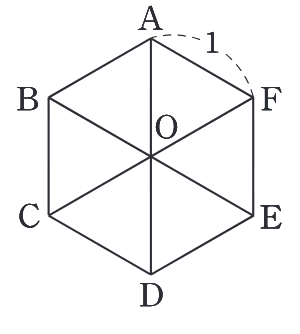
\includegraphics[width=\dmfigw]{figures/fig-147-e1.png}\end{minipage}\par
\dmsubprob{1} $\overrightarrow{\pt{DE}}$와 서로 같은 벡터를 모두 구하시오.
\dmsubprob{2} $\overrightarrow{\pt{BC}}$와 크기가 같고 방향이 반대인 벡터를 모두 구하시오.
\dmsubprob{3} $\overrightarrow{\pt{BC}}$의 크기를 구하시오.
\dmsubprob{4} $|\overrightarrow{\pt{AE}}|$를 구하시오.
